\chapter{Virtualization Architecture}\label{ch:2-virtualization-architecture}

\section{Architecture Overview}\label{sec:2-1}

RVM is a virtual machine monitor built specifically for resource-constrained microcontrollers. It can decompose a single microcontroller into multiple virtual microcontrollers that do not affect one another in time or space. Even if one of the virtual microcontrollers suffers a fatal failure, the other virtual microcontrollers can still operate normally and are not adversely affected, thereby effectively preventing faults or security vulnerabilities from spreading throughout the entire system.

Unlike common products such as KVM, Virtual
Box, and VMWare, RVM statically allocates the microcontroller's resources to each virtual microcontroller, and the resource allocation information can be determined at system compile time. Three important factors led to this design: (1) the vast majority of microcontrollers rely on Flash memory to store programs and lack the ability to load dynamic runtime libraries, (2) microcontrollers have very few resources and must use them extremely efficiently, so they can hardly bear the extra overhead brought by dynamic data structures, and (3) introducing too much dynamism into critical systems may make system behavior difficult to predict. Of course, within each virtual microcontroller, features such as dynamic memory allocation and dynamic thread creation can still be used; even if these dynamic behaviors cause a virtual microcontroller to fail, they will not affect the normal operation of the other virtual microcontrollers.

Another difference between RVM and conventional virtualization solutions is that its guests run real-time operating systems (Real-Time
Operating
System, RTOS). These operating systems have two characteristics: (1) they require system latency to be deterministic, and (2) they require the virtualization overhead to be very low. Conventional virtualization solutions are often based on operation\footnote{or binary} translation, and their underlying primitives often deviate somewhat from the interface semantics of the guest operating system; a simple guest request may be translated into a large number of hypercalls (Hypercall), causing latency amplification of hundreds of times. To solve this problem, RVM (1) designs all code inside it according to real-time system standards, with deterministic execution latency, and (2) designs its internal operation primitives and hypercall semantics to be RTOS-friendly, so that an RTOS operation is translated into only one operation primitive or hypercall.

The last difference between RVM and conventional virtualization solutions is that it often faces (extremely) stringent memory requirements. These requirements are quite extreme\footnote{in some cases even tens or just a few bytes must be fought for}, but they are not incomprehensible: any CPU and memory overhead used for resource isolation can be saved in designs that do not value product quality; yet microcontrollers are very inexpensive and used in very high volumes, so any increase in cost is greatly reflected in the final selling price of the product; if the isolation overhead is so high that even a slightly more expensive microcontroller is required, the loss outweighs the gain. For this reason, RVM is designed to be extremely memory-frugal. It needs only a minimum of 5kB
RAM and 20kB
ROM to run, and may therefore be the smallest virtualization environment in the world. This allows it to be widely used on those mainstream microcontroller families with 128kB
ROM and 64kB RAM, as long as they have a memory protection unit (Memory
Protection Unit, MPU).

To meet the above challenges, RVM requires a large amount of address information to be determined statically at system compile time and creates a series of kernel objects with specific parameters. The corresponding data structures are also specially designed, which makes filling them in by hand very difficult. For this reason, RVM also provides a project generator, which can generate from the description of the system the initialization code, linker scripts, and even project files corresponding to the relevant build environment that the project requires.

Thus, the RME microkernel, the RVM monitor, the native processes and various RTOS virtual machines running on it, and the project generator used to generate the entire project constitute the RME microcontroller operating system ecosystem. The overall virtualization architecture is shown in the figure below: solid lines in the figure represent hardware isolation mechanisms, and dashed lines represent the boundaries of software modules.


\begin{figure}[htbp]
\centering
\resizebox{\textwidth}{!}{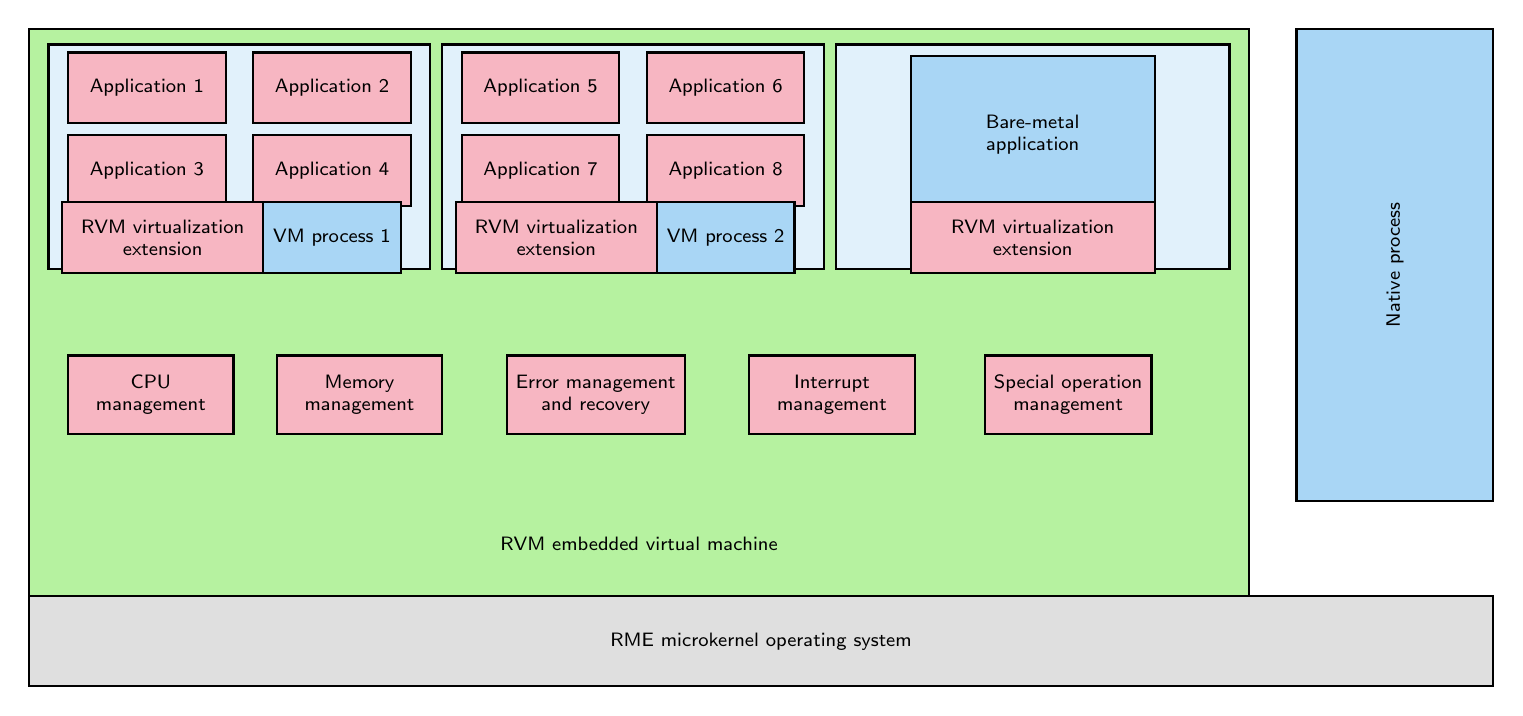
\begin{tikzpicture}[x=1cm,y=1cm,font=\sffamily\scriptsize,
    app/.style={draw,thick,fill=rvmpink,minimum width=2.0cm,minimum height=0.9cm,align=center},
    ext/.style={draw,thick,fill=rvmpink,minimum width=2.4cm,minimum height=0.9cm,align=center},
    vm/.style={draw,thick,fill=rvmblue,minimum width=2.0cm,minimum height=0.9cm,align=center},
    mgmt/.style={draw,thick,fill=rvmpink,minimum width=2.1cm,minimum height=1.0cm,align=center},
    proc/.style={draw,thick,fill=rvmblue,minimum width=2.1cm,minimum height=6.0cm,align=center}]
\definecolor{rvmgreenbg}{RGB}{182,242,160}
\definecolor{rvmpink}{RGB}{247,182,194}
\definecolor{rvmblue}{RGB}{169,214,245}
% RVM green container
\fill[rvmgreenbg] (0,0) rectangle (15.5,7.2);
\draw[thick] (0,0) rectangle (15.5,7.2);
% Three VM columns
\foreach \x/\base/\name in {0.25/1/1, 5.25/5/2} {
  \draw[thick,fill=rvmblue!35] (\x,4.15) rectangle (\x+4.85,7.0);
  \node[app] at (\x+1.25,6.45) {Application \base};
  \node[app] at (\x+3.60,6.45) {Application \the\numexpr\base+1\relax};
  \node[app] at (\x+1.25,5.40) {Application \the\numexpr\base+2\relax};
  \node[app] at (\x+3.60,5.40) {Application \the\numexpr\base+3\relax};
  \node[ext,minimum width=2.55cm] at (\x+1.45,4.55) {RVM virtualization\\extension};
  \node[vm,minimum width=1.75cm] at (\x+3.60,4.55) {VM process \name};
}
% Bare-metal column
\draw[thick,fill=rvmblue!35] (10.25,4.15) rectangle (15.25,7.0);
\node[fill=rvmblue,draw,thick,minimum width=3.1cm,minimum height=2.0cm,align=center] at (12.75,5.85) {Bare-metal\\application};
\node[ext,minimum width=3.1cm] at (12.75,4.55) {RVM virtualization\\extension};
% Management row
\node[mgmt] at (1.55,2.55) {CPU\\management};
\node[mgmt] at (4.20,2.55) {Memory\\management};
\node[mgmt] at (7.20,2.55) {Error management\\and recovery};
\node[mgmt] at (10.20,2.55) {Interrupt\\management};
\node[mgmt] at (13.20,2.55) {Special operation\\management};
\node[anchor=south] at (7.75,0.45) {RVM embedded virtual machine};
% Native process
\draw[thick,fill=rvmblue] (16.1,1.2) rectangle (18.6,7.2);
\node[rotate=90] at (17.35,4.2) {Native process};
% RME bar
\fill[gray!25] (0,-1.15) rectangle (18.6,0);
\draw[thick] (0,-1.15) rectangle (18.6,0);
\node at (9.3,-0.58) {RME microkernel operating system};
\end{tikzpicture}
}
\caption{Simplified diagram of the RVM architecture}\label{fig:2-1}
\end{figure}


RVM virtual machines run on a virtual machine monitor implemented on the basis of paravirtualization technology. It implements all the basic functions of virtualization: memory management, CPU management, interrupt vector virtualization, and virtual machine error handling. For specific information about these implementations, see the following sections.

\subsection{RME Microkernel}\label{subsec:2-1-1}

The RME microkernel exists as the underlying support for RVM and is responsible for providing basic operating system services to RVM. All other components running on the microcontroller exist as RME processes. For information about the RME microkernel, see the relevant kernel documentation.

\subsection{RVM Virtual Machine Monitor}\label{subsec:2-1-2}

The RVM virtual machine monitor is responsible for the concrete virtual machine management work and runs on RME as a Type II virtual machine monitor. Specifically, it delivers physical interrupts and event source signals to each virtual machine and responds to hypercall requests from each virtual machine. When a virtual machine encounters an exception, RVM is also responsible for restarting the corresponding virtual machine. The virtual machine monitor includes five daemon threads: the initialization daemon (Initialization
Daemon, INIT), the safety daemon coroutine (Safety Daemon, SFTD), the timer
daemon coroutine (Timer
Daemon, TIMD), the vector daemon coroutine (Vector
Daemon, VCTD), and the hypercall daemon thread (Hypercall
Daemon, HYPD); the latter three coroutines all run together on top of the virtual machine monitor daemon (Virtual
Machine Monitor Daemon, VMMD). The following introduces these five daemon threads one by one.

\subsubsection{Startup Daemon Thread INIT}\label{subsubsec:2-1-2-1}

INIT is created by RME at startup; it is responsible for initializing the native threads and virtual machines in the system and for starting the remaining four daemon threads. After this work is complete, INIT goes to sleep and is scheduled only when there is no runnable thread in the system. Once it is scheduled, it repeatedly executes the processor sleep instruction, putting the processor into a low-power state to wait for interrupts.

\subsubsection{Safety Daemon Coroutine SFTD}\label{subsubsec:2-1-2-2}

SFTD runs at the highest priority in the system\footnote{Kern\_Prio-1} and is responsible for monitoring the operation of native processes and virtual machines. It normally blocks on the error handling endpoint RVM\_Sftd\_Sig\_Cap; once any exception occurs in a native process or virtual machine, SFTD unblocks and starts running. If the exception occurred in a native process, SFTD restarts the entire system; if the exception occurred in a virtual machine, SFTD restarts only that virtual machine.

\subsubsection{Vector Daemon Coroutine VCTD}\label{subsubsec:2-1-2-3}

VCTD runs at a priority lower than native processes but higher than virtual machines, and is responsible for forwarding physical interrupts and event activations in the system to the interrupt sources of each virtual machine. It normally blocks on the interrupt vector endpoint RVM\_BOOT\_INIT\_VCT; once this endpoint receives any signal, VCTD unblocks and starts running. VCTD extracts interrupt vector and event source activation information from the two RVM\_Flag data structures located at RVM\_PHYS\_VCT\_BASE and RVM\_VIRT\_EVT\_BASE respectively, and forwards it to the virtual machines.

Each RVM\_Flag data structure is formed by combining two identical struct
\_\_RME\_RVM\_Flag structures. This is because VCTD requires exclusive access to the struct
\_\_RME\_RVM\_Flag when accessing it, and at that time, if the kernel needs to pass activation information to RVM, it can only choose to fill the other copy of the structure. Each structure contains the following three fields:

\begin{xltabular}{\textwidth}{@{}>{\hsize=0.4500\hsize\raggedright\arraybackslash}X>{\hsize=1.5500\hsize\raggedright\arraybackslash}X@{}}
\caption{Meaning of each field in struct \_\allowbreak{}\_\allowbreak{}RME\_\allowbreak{}RVM\_\allowbreak{}Flag}\label{tab:2-1}\\
\toprule
Field name & Purpose\tabularnewline
\endfirsthead
\toprule
Field name & Purpose\tabularnewline
\midrule
\endhead
\bottomrule
\endlastfoot
ptr\_\allowbreak{}t Lock &
Determines whether this structure is currently being used by VCTD. If VCTD is using the structure, the kernel cannot operate on it; otherwise a race condition may occur. The kernel will then choose to fill the other structure.\tabularnewline
ptr\_\allowbreak{}t Fast &
Indicates activation of a fast signal source. If it is 1, the fast interrupt source is activated. Currently, this field is used only in the structure located at RVM\_\allowbreak{}PHYS\_\allowbreak{}VCT\_\allowbreak{}BASE, to convey the clock interrupt signal.\tabularnewline
ptr\_\allowbreak{}t Group &
Indicates the group of an activated slow signal source; it is a bitmap. If a bit is set, it means that a signal in that group in the Flag field has been activated: if bit 2 is set, it means that a bit of Flag{[}2{]} is nonzero. The purpose of setting this field is to quickly find the group in which the activated signal is located.\tabularnewline
ptr\_\allowbreak{}t Flag{[}{]} &
A bitmap indicating the specific activated signal sources. Its length is determined by the number of signals: if the word length of the processor is 32 bits and there are 96 interrupt sources, the length of this field is 96/32=3 machine words.\tabularnewline
\end{xltabular}

For example, on a 32-bit processor, if physical interrupt source 34 is activated, the kernel first searches the two struct
\_\_RME\_RVM\_Flag structures located at RVM\_PHYS\_VCT\_BASE and selects the copy whose Lock field is 0. The kernel then sets bit {[}2{]} of Flag{[}1{]} and sets bit {[}1{]} of Group. Finally, the kernel sends a signal to RVM\_BOOT\_INIT\_VCT to activate VCTD. After VCTD is activated, it alternately searches the two struct
\_\_RME\_RVM\_Flag structures for set bits. When searching, it first sets the Lock of the first struct
\_\_RME\_RVM\_Flag to 1, then queries which bits in Group are set, and uses that information to query the corresponding Flag{[}{]}, obtaining the specific interrupt source number. If interrupt source 34 is the one activated, it should find bit {[}1{]} of Group set and then query Flag{[}1{]}; in Flag{[}1{]} it finds its bit {[}2{]} set. From this, VCTD can deduce that the activated interrupt source is number 34 and activate those virtual machines that have registered physical interrupt source 34. For information about activating virtual machines, see \protect\hyperref[subsec:2-2-4]{2.2.4}.

The activation process for event sources is similar to the activation process for physical interrupt sources. For information about event sources, see \protect\hyperref[subsec:2-2-7]{2.2.7}.

\subsubsection{Timer Daemon Coroutine TIMD}\label{subsubsec:2-1-2-4}

The timer daemon thread TIMD runs at the same priority as VCTD and is responsible for delivering RVM clock ticks to each virtual machine. It normally blocks on the clock interrupt endpoint RVM\_BOOT\_INIT\_VCT, and once the endpoint receives a timer interrupt, it delivers that interrupt to all virtual machines. Each signal TIMD receives on the clock interrupt endpoint RVM\_BOOT\_INIT\_VCT counts as one RVM clock tick. Each virtual machine can specify a frequency division factor Period\footnote{see \protect4.2}, and only after Period RVM clock ticks have been received is a virtual clock interrupt sent to the virtual machine.

The timer daemon thread also allows a watchdog timeout Watchdog\footnote{see \protect4.2} to be specified for each virtual machine. A virtual machine can use the hypercall RVM\_Hyp\_Wdg\_Clr to feed the watchdog; if the virtual machine has still not fed the watchdog after Watchdog ticks, it is determined that the virtual machine is stuck in an infinite loop, and TIMD will restart it.

\subsubsection{Hypercall Daemon Coroutine HYPD}\label{subsubsec:2-1-2-5}

The hypercall daemon thread HYPD runs at the same priority as VCTD and is responsible for receiving and handling hypercalls sent by the virtual machines. It normally blocks on the hypercall handling endpoint RVM\_BOOT\_INIT\_VCT, and once the endpoint receives a signal, it handles the hypercall initiated by the current virtual machine. For the specific handling method of hypercalls, see \protect\hyperref[subsec:2-2-6]{2.2.6}.

\needspace{14\baselineskip}
\subsection{Protection Domains}\label{subsec:2-1-3}

\needspace{10\baselineskip}
RVM provides two kinds of protection domains, namely native processes and virtual machines. A brief comparison of the two is as follows:

\begin{xltabular}{\textwidth}{@{}>{\hsize=1.2000\hsize\raggedright\arraybackslash}X*{8}{>{\hsize=0.9750\hsize\centering\arraybackslash}X}@{}}
\caption{Comparison between native processes and virtual machines}\label{tab:2-2}\\
\toprule
\rule{0pt}{3.1cm}\rotatebox{90}{Protection domain} & \rotatebox{90}{Confidentiality} & \rotatebox{90}{Integrity} & \rotatebox{90}{Availability} & \rotatebox{90}{Auditability} & \rotatebox{90}{Real-time} & \rotatebox{90}{Compactness} & \rotatebox{90}{Reliability}
& \rotatebox{90}{Usability}\tabularnewline
\endfirsthead
\toprule
\rule{0pt}{3.1cm}\rotatebox{90}{Protection domain} & \rotatebox{90}{Confidentiality} & \rotatebox{90}{Integrity} & \rotatebox{90}{Availability} & \rotatebox{90}{Auditability} & \rotatebox{90}{Real-time} & \rotatebox{90}{Compactness} & \rotatebox{90}{Reliability}
& \rotatebox{90}{Usability}\tabularnewline
\midrule
\endhead
\bottomrule
\endlastfoot
Native process & Strong & Weak & Weak & Weak & Strong & Strong & Weak & Weak\tabularnewline
Virtual machine & Strong & Strong & Strong & Strong & Weak & Weak & Strong & Strong\tabularnewline
\end{xltabular}

\subsubsection{Native Process}\label{subsubsec:2-1-3-1}

RME native processes run directly on the RME microkernel. They are not constrained by the RVM virtual machine monitor, and their resource consumption is lower than that of virtual machines. They are mainly used to receive signals from interrupt vectors and, after preliminary processing, forward these signals to virtual machines. The timeslices of threads in native processes are all unlimited, and they have the highest priority in the entire system. Even if RVM and all the virtual machines it manages have crashed, the threads in native processes can still run normally, thereby maintaining the safety of the controlled equipment.

Even though native processes are not virtual machines, the project generator still provides complete support for them, and the RVM user-mode library also provides a series of wrappers around system calls to facilitate their use in C programs. The project generator can even generate a project containing no virtual machines; in this case, application functionality can only be implemented using native processes and system calls.

RVM does not provide fault tolerance for native processes; if an exception occurs in any native process, RVM's SFTD considers that a serious problem has occurred in the system and restarts the entire system. Therefore, native processes possess only confidentiality among the three elements of security; once compromised, the integrity and availability of the system are completely lost.

\subsubsection{Virtual Machine}\label{subsubsec:2-1-3-2}

Each RVM virtual machine is a separate process, inside which the hardware abstraction layer on which the RTOS depends at runtime can be emulated. It has an interrupt vector thread Vct and a user program thread Usr to emulate processor interrupts and the normal program execution flow respectively: to facilitate the RTOS's software interrupt thread switching, the Usr thread can directly trigger the running of the Vct thread, and the Vct thread can directly modify the register set of the Usr thread.

In RVM-based systems, it is recommended to implement any moderately complex functionality in virtual machines, especially language virtual machines, graphical user interfaces, and the like. This is not only because the RTOS in a virtual machine provides a series of libraries, possible POSIX support, and certified software, but also, more importantly, because a virtual machine automatically restarts only itself rather than the entire system after a fault occurs. This is crucial for fault isolation in functional safety.

A virtual machine can access a series of special virtualization-related features through hypercalls, including interrupt management, event source management and communication, etc. These hypercalls are intercepted and responded to by RVM's HYPD.

\subsection{Project Generator}\label{subsec:2-1-4}

The project generator provided by RVM can generate a compilable project from a project description file. It can automatically calculate and allocate the addresses of each kernel object and generate the corresponding configuration files, without the user needing to make any manual adjustments.

\section{Virtualization Principles}\label{sec:2-2}

After RVM starts, the first to execute is the startup daemon thread INIT. It loads each virtual machine and is responsible for starting the safety daemon thread, the vector daemon thread, the hypercall daemon thread, and the timer daemon thread. Among them, the safety daemon thread restarts a virtual machine when an error occurs in it\footnote{RVM does not natively support user-defined error handling}; the vector daemon thread redirects physical interrupts from devices or event source activations to the virtual interrupt vectors of the corresponding virtual machine; the hypercall daemon thread is responsible for handling hypercalls and virtual machine scheduling; and the timer daemon thread is responsible for sending clock interrupts to each virtual machine.

Inside each virtual machine, two threads run: one is responsible for handling interrupts inside the virtual machine, and the other is responsible for running user code. The specific virtualization principles are introduced in the following subsections.

\subsection{Priority Configuration}\label{subsec:2-2-1}

In RVM, the safety daemon thread SFTD always runs at the highest priority in the system. Immediately following it are the threads in native processes, which are responsible for quickly handling some interrupts in the system that cannot be sent to virtual machines in time. Next are the three daemon threads VCTD, TIMD, and HYPD, which run at a priority lower than native processes but higher than virtual machines. Then come the interrupt handling thread Vct and the user thread Usr of running virtual machines, with Vct having a higher priority than Usr. After that is the system's own INIT process, which is responsible for calling the idle hook in an infinite loop, putting the system to sleep when no virtual machine is ready. Finally come the interrupt handling threads and user program threads of virtual machines that are not running. The interrupt priorities of the threads in the entire virtualization architecture are as follows:


\begin{figure}[htbp]
\centering
\resizebox{\textwidth}{!}{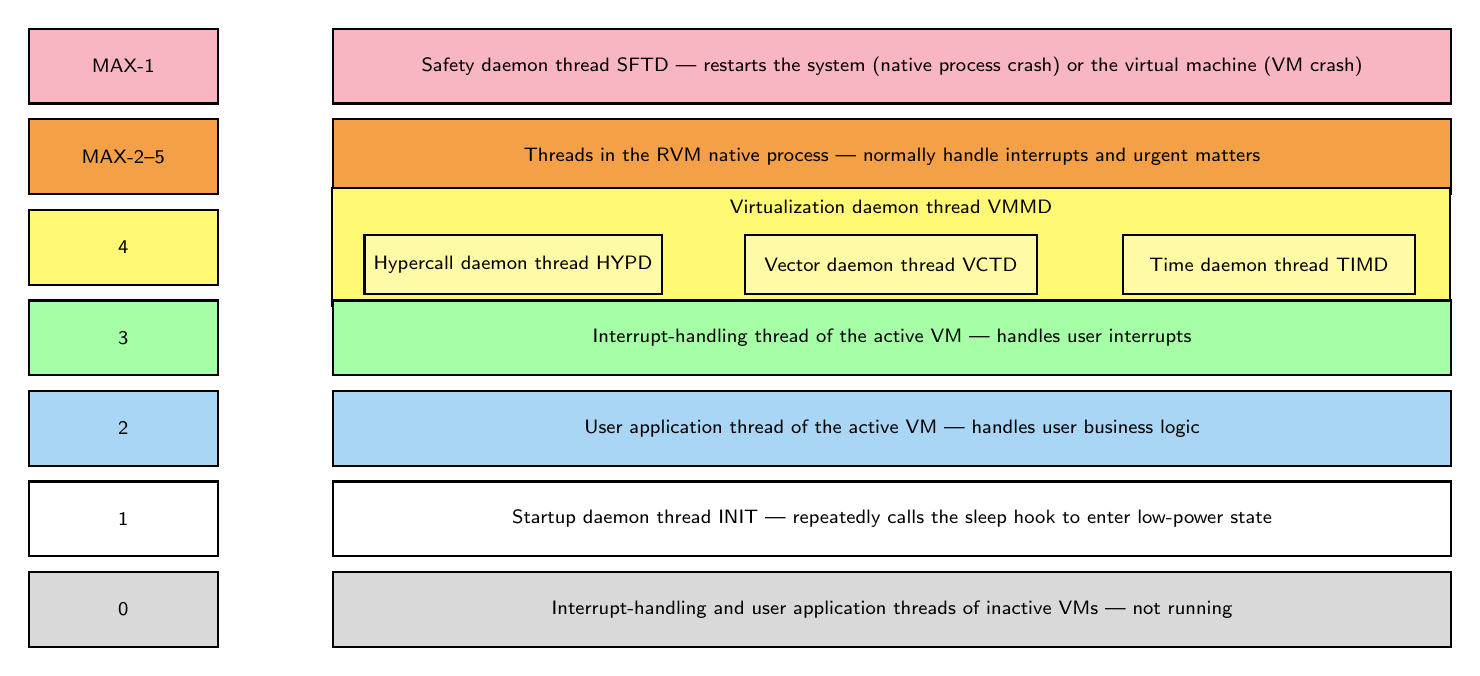
\begin{tikzpicture}[x=1cm,y=1cm,font=\sffamily\scriptsize,
    prio/.style={draw,thick,minimum width=2.4cm,minimum height=0.95cm,align=center},
    bar/.style={draw,thick,minimum height=0.95cm,align=center},
    daemon/.style={draw,thick,fill=yellow!35,minimum height=0.75cm,align=center}]
\definecolor{rvmpink}{RGB}{247,182,194}
\definecolor{rvmblue}{RGB}{169,214,245}
\definecolor{rvmorange}{RGB}{244,160,70}
% Priority rows, top to bottom
\node[prio,fill=rvmpink] (p1) at (0,0) {MAX-1};
\node[bar,fill=rvmpink,minimum width=14.2cm,anchor=west] at (2.65,0) {Safety daemon thread SFTD --- restarts the system (native process crash) or the virtual machine (VM crash)};
\node[prio,fill=rvmorange] at (0,-1.15) {MAX-2--5};
\node[bar,fill=rvmorange,minimum width=14.2cm,anchor=west] at (2.65,-1.15) {Threads in the RVM native process --- normally handle interrupts and urgent matters};
\node[prio,fill=yellow!55] at (0,-2.30) {4};
\draw[thick,fill=yellow!55] (2.65,-1.55) rectangle (16.85,-3.05);
\node at (9.75,-1.78) {Virtualization daemon thread VMMD};
\node[daemon,minimum width=3.7cm] at (4.95,-2.52) {Hypercall daemon thread HYPD};
\node[daemon,minimum width=3.7cm] at (9.75,-2.52) {Vector daemon thread VCTD};
\node[daemon,minimum width=3.7cm] at (14.55,-2.52) {Time daemon thread TIMD};
\node[prio,fill=green!35] at (0,-3.45) {3};
\node[bar,fill=green!35,minimum width=14.2cm,anchor=west] at (2.65,-3.45) {Interrupt-handling thread of the active VM --- handles user interrupts};
\node[prio,fill=rvmblue] at (0,-4.60) {2};
\node[bar,fill=rvmblue,minimum width=14.2cm,anchor=west] at (2.65,-4.60) {User application thread of the active VM --- handles user business logic};
\node[prio,fill=white] at (0,-5.75) {1};
\node[bar,fill=white,minimum width=14.2cm,anchor=west] at (2.65,-5.75) {Startup daemon thread INIT --- repeatedly calls the sleep hook to enter low-power state};
\node[prio,fill=gray!30] at (0,-6.90) {0};
\node[bar,fill=gray!30,minimum width=14.2cm,anchor=west] at (2.65,-6.90) {Interrupt-handling and user application threads of inactive VMs --- not running};
\end{tikzpicture}
}
\caption{Interrupt priorities in the virtualization architecture}\label{fig:2-2}
\end{figure}


The virtual machines are scheduled using a fixed-priority timeslice round-robin method. The priorities among them are determined by the scheduler daemon thread. For system safety, the timeslices and priorities of virtual machines are statically determined at system compile time, and RVM does not provide hypercalls that can modify these two. This fundamentally guarantees time isolation between virtual machines, so that no virtual machine can compromise the real-time performance of the entire system.

\subsection{Memory Management}\label{subsec:2-2-2}

In virtual machines, one of the most important matters is memory management. Considering the general characteristics of microcontroller applications, each virtual machine's private memory and shared memory are statically specified at compile time. After the system starts running, modification of the memory mapping is no longer allowed. For each type of processor, the format of page table information is different. Please refer to the corresponding processor's user manual to determine the page table format of that processor.

Constructing and filling in page tables by hand is very tedious; to avoid unnecessary trouble, the project generator provides functions for automatically constructing and filling in page tables.

\subsection{CPU Virtualization}\label{subsec:2-2-3}

In different paravirtualization platforms, CPU virtualization mainly has two mainstream design strategies, as follows:

\begin{enumerate}
\def\labelenumi{{[}\arabic{enumi}{]}}
\item
  Run each virtual machine as a single thread. This is the most common solution on dedicated paravirtualization platforms; Xen adopts this strategy. In each guest, the thread normally executes application code; once a device interrupt or exception occurs\footnote{On x86, Xen uses the hardware-specific Ring1 to accelerate system call and exception handling without going through Xen, but device interrupts still need to be distributed through Xen}, the virtual machine monitor forcibly modifies the thread's execution address, forcing it to execute a piece of interrupt handling code, and after handling is finished, the thread returns by itself to execute in the application. From the virtual machine monitor's point of view, this method is the most convenient: on the one hand, each guest has only one execution context; on the other hand, activating an interrupt requires only modifying that context's instruction pointer. However, from the guest's point of view, the question of whether the end of interrupt (End-Of-Interrupt, EOI) needs to specifically notify the virtual machine monitor becomes difficult to handle. There are mainly two cases: the relatively simple case (1) in which, once the virtual machine monitor has forced a guest to execute a virtual interrupt vector, the virtual machine monitor must not modify the instruction pointer again to force the virtual machine to execute an interrupt vector until the guest uses a dedicated hypercall to notify the virtual machine monitor that the current interrupt has ended; and the more complex case (2) in which the virtual machine monitor always modifies the instruction pointer to force the virtual machine to execute an interrupt vector, regardless of whether the guest is executing a virtual interrupt vector. In case (1), the guest side needs to invoke a hypercall to notify the virtual machine, which undoubtedly adds one hypercall. For a native virtual machine monitor such as Xen, which runs directly in privileged mode, one hypercall is one context switch, and the overhead is still tolerable; for a hosted virtual machine monitor such as RVM, which runs in user mode, one hypercall means two context switches, and the introduced latency cannot be ignored. If the solution in case (2) is adopted, it is even worse: this means that the interrupt vector entry must be reentrant, and therefore requires a very special piece of assembly code. This code must be responsible for recognizing reentrancy before the reentrant execution instance reaches the real interrupt vector and then voluntarily exiting; the exit process must also involve patching the stack frame so that the execution flow returns to the interrupt vector being executed with the correct stack pointer. On the one hand, this code is very difficult to write correctly\footnote{this is even more so for the wide variety of non-standard embedded architectures}; on the other hand, its beginning is always a large block of pushes onto the stack. If a series of closely consecutive interrupts occurs, the push code at the beginning will reenter multiple times before stack frame patching can be performed, potentially causing a stack overflow in an embedded environment. Therefore, even though (2) is very efficient in Xen, we do not adopt this approach.
\item
  Run every thread in each guest as an independent virtual machine thread. This is a common solution for microkernel-based virtualization; L4Linux adopts this strategy\protect\hyperref[cite:2-2]{{[}2{]}}. On microcontrollers, the problems with this strategy are: (1) the original guest operating system's thread interface must somehow be connected to the microkernel's system calls, which requires a full understanding of the original operating system's design and may even involve modifications to architecture-independent parts such as thread control blocks; (2) mapping every guest thread to a microkernel thread creates a large number of microkernel thread objects, which is not a problem in heavyweight operating systems such as Linux whose thread structures are already large, but in RTOSes whose threads are generally extremely lightweight it amounts to multiplying memory consumption; (3) a microkernel thread switch requires a series of operation capability checks, time budget checks, and protection domain switch checks, while RTOS threads that do not even have protection domains do not need these checks at all, so calling the microkernel system call for every thread switch amounts to multiplying execution time consumption, and this is even more so on those microkernels that treat time resources as independently allocatable resources\footnote{such as Composite and some L4 variants}.

  To resolve the above dilemma, RVM uses a dual-thread approach for guest CPU virtualization. Each guest has two threads, Vct and Usr; the Vct thread is responsible for interrupt handling, and the Usr thread is responsible for handling user programs. Vct normally does not run and runs only when it receives an interrupt trigger signal from RVM. After interrupt handling is complete, Vct blocks again and Usr starts running. The switch from Vct to Usr uses the microkernel's efficient asynchronous signal mechanism and does not involve RVM, so it is much faster than a hypercall.

  When Usr is switched out, its register set is saved at the address specified by Reg\_Base\footnote{see \protect4.2}. Therefore, to modify Usr's register set in Vct, it is sufficient to modify the register data at that address. Using this method, without needing to understand the original RTOS design, one can replace its hardware abstraction layer, especially its thread switching assembly, line by line, thereby easily emulating the thread context switching that is very common in RTOSes.
\end{enumerate}

\subsection{Interrupt Virtualization}\label{subsec:2-2-4}

For virtual machines, interrupt virtualization is indispensable. Each RVM guest has an interrupt handling thread Vct, whose priority is higher than that of the Usr thread that handles user programs. This thread normally blocks on the virtual interrupt vector endpoint dedicated to each virtual machine\footnote{this endpoint is located at capability number 1 inside each virtual machine}, and is woken up to run only when a virtual interrupt signal from RVM is received.

Interrupts in the system can roughly be divided into three categories: the first is clock interrupts, which are responsible for providing ticks to the operating system; the second is thread switching interrupts, which are responsible for RTOS thread switching; and the third is other system interrupts, which are responsible for responding to transactions of other peripherals. The characteristics of these three categories also differ: clock interrupts occur periodically and frequently; thread switching interrupts are essentially software interrupts sent by a thread to itself; and other system interrupts are irregular interrupts that occur from time to time. Therefore, RVM adopts different virtualization strategies for these three kinds of interrupts.

Each virtual machine maintains an RVM\_State data structure, whose address is specified by State\_Base\footnote{see \protect4.2}. Its internal fields are as follows:

\begin{xltabular}{\textwidth}{@{}>{\hsize=0.4500\hsize\raggedright\arraybackslash}X>{\hsize=1.5500\hsize\raggedright\arraybackslash}X@{}}
\caption{Meaning of each field in struct RVM\_\allowbreak{}State}\label{tab:2-3}\\
\toprule
Field name & Purpose\tabularnewline
\endfirsthead
\toprule
Field name & Purpose\tabularnewline
\midrule
\endhead
\bottomrule
\endlastfoot
ptr\_\allowbreak{}t Vct\_\allowbreak{}Act &
Indicates the thread currently running in the virtual machine. If set to 1, the Vct thread is running; otherwise, the Usr thread is running.\tabularnewline
struct RVM\_\allowbreak{}Param Vct & Hypercall parameter area dedicated to the Vct thread.\tabularnewline
struct RVM\_\allowbreak{}Param Usr & Hypercall parameter area dedicated to the Usr thread.\tabularnewline
struct RVM\_\allowbreak{}Vctf Flag &
Indicates the virtual interrupt vectors activated in the current virtual machine.\tabularnewline
\end{xltabular}

In this data structure, the data structure related to interrupt virtualization is struct RVM\_Vctf Flag, whose fields are shown in the following table. For the other fields, see \protect\hyperref[subsec:2-2-6]{2.2.6}.

\begin{xltabular}{\textwidth}{@{}>{\hsize=0.4500\hsize\raggedright\arraybackslash}X>{\hsize=1.5500\hsize\raggedright\arraybackslash}X@{}}
\caption{Meaning of each field in struct RVM\_\allowbreak{}Vctf}\label{tab:2-4}\\
\toprule
Field name & Purpose\tabularnewline
\endfirsthead
\toprule
Field name & Purpose\tabularnewline
\midrule
\endhead
\bottomrule
\endlastfoot
ptr\_\allowbreak{}t Tim & Indicates clock interrupt activation.\tabularnewline
ptr\_\allowbreak{}t Ctx & Indicates thread switching interrupt activation.\tabularnewline
u8\_\allowbreak{}t Vct{[}{]} &
Indicates activation of other virtual interrupt vectors. Each byte corresponds to one virtual interrupt vector.\tabularnewline
\end{xltabular}

In this data structure, activation of the clock interrupt and the thread switching interrupt is indicated by two separate machine words, while each of the other virtual interrupt vectors corresponds to one byte. When the corresponding interrupt is activated, the corresponding field is set to 1. Here, the method of one binary bit per interrupt vector is not adopted, so that no atomic logical AND instruction is needed\footnote{When VCTD sets a vector, the Vct thread may be resetting one of the vectors. If one binary bit corresponded to one interrupt vector, the Vct thread would have to use an atomic logical AND operation to reset the flag bit. Some architectures, such as ARMv6-M, do not have such an atomic operation, so one byte per flag offers better compatibility.}. Since the number of virtual interrupt vectors of each virtual machine is limited, the resulting waste of storage space is tolerable.

For example, if VCTD determines that interrupt vector 4 of a virtual machine is activated, it sets Vct{[}4{]} to 1 and sends a signal to the dedicated endpoint of that virtual machine's Vct thread. After the Vct thread receiving the signal is activated, it first scans the entire structure and determines that virtual interrupt vector 4 is activated from Vct{[}4{]} being set to 1. After that, the Vct thread first clears Vct{[}4{]} to zero and then invokes virtual interrupt vector 4 registered by the user using RVM\_Virt\_Vct\_Reg\footnote{see \protect4.5.5}. In this way, even if a new interrupt 4 arrives while the user-registered interrupt vector is executing, no interrupt loss occurs, because Vct{[}4{]} will be set again: after the next loop, the Vct thread will detect that interrupt 4 is pending and enter it again.

A virtual machine's interrupt enable/disable, as well as the correspondence between the virtual machine's virtual interrupt vectors and the corresponding physical interrupt vectors or event sources, can be set through hypercalls. For information about these hypercalls, see \protect\hyperref[sec:4-4]{4.4}. A standard virtual machine interrupt initialization flow is as follows:

\begin{enumerate}
\def\labelenumi{{[}\arabic{enumi}{]}}
\item
  Call RVM\_Virt\_Tim\_Reg to register the clock interrupt,
\item
  Call RVM\_Virt\_Ctx\_Reg to register the thread switching interrupt,
\item
  Call RVM\_Virt\_Vct\_Reg to register other virtual interrupts,
\item
  Call RVM\_Hyp\_Vct\_Phys to map the required physical interrupt sources to virtual interrupt sources,
\item
  Call RVM\_Hyp\_Vct\_Evt to map the required event sources to virtual interrupt sources,
\item
  Call RVM\_Hyp\_Vct\_Lck to lock the event source mappings to prevent subsequent tampering,
\item
  Call RVM\_Hyp\_Int\_Ena at an appropriate place to enable the virtual machine's global interrupts. If the virtual machine also uses a watchdog, RVM\_Hyp\_Wdg\_Clr needs to be called to start the watchdog. Once started, the watchdog cannot be disabled.
\item
  The RTOS inside the virtual machine should repeatedly call RVM\_Hyp\_Vct\_Wait in its idle thread so that the virtual machine enters sleep when idle and waits for the next interrupt. If the virtual machine also uses a watchdog, RVM\_Hyp\_Wdg\_Clr needs to be called at an appropriate place to feed the watchdog.
\end{enumerate}

\subsubsection{Virtualization of Timer Interrupts}\label{subsubsec:2-2-4-1}

RTOSes running on RVM can be divided into two categories according to the way they use timers: periodic kernels and tickless kernels. The former requires the system to have an auto-reload timer that periodically sends interrupts, while the latter requires programming, as needed on each context switch, a one-shot timer that sends an interrupt after a countdown ends. On bare metal, the latter is superior in terms of low-power characteristics, because no clock interrupt is generated when the processor is sleeping or only one task is scheduled. For this reason, we often enable this feature on RTOSes that support tickless kernels.

However, in a virtualization environment the situation is exactly the opposite. A tickless kernel can no longer program the timer directly; it must ask RVM for help through a hypercall. This results in an extra hypercall on every context switch, causing intolerable performance and real-time overhead. In addition, not all RTOSes support tickless kernel mode: even if only one periodic kernel runs on RVM, RVM still has to be woken up periodically to send timer interrupts to it, so reducing power consumption is impossible; this makes the tickless feature of other kernels add only overhead. Even setting that aside, even if all virtual machines running on RVM are tickless, the total number of times they program the timer would still be very large, and RVM must set the hardware timer's timeout to the minimum of all these times. This causes the timer to always be triggered after a short period of time, and is also unlikely to achieve a low-power effect.

For the above reasons, RVM uses a periodic design. The periodic clock signal it needs is generated by the RME underlying timer and sent to RVM's clock handling daemon thread through the RVM\_BOOT\_INIT\_TIM endpoint. This daemon thread calculates the number of time periods currently elapsed and sends clock interrupts to each virtual machine according to the frequency division factor Period\footnote{see \protect4.2} configured for each virtual machine.

Specifically, the Vct thread calls the thread switching hook Tim registered by the user using RVM\_Virt\_Tim\_Reg\footnote{see \protect4.5.7}. This hook function can directly use the timer interrupt vector of the original bare-metal RTOS, and when needed can use RVM\_Virt\_Yield\footnote{see \protect4.5.7} to trigger a context switch\footnote{just as a context switching interrupt such as PendSV is triggered in the original RTOS}.

\subsubsection{Virtualization of Thread Switching Interrupts}\label{subsubsec:2-2-4-2}

A thread switching interrupt is essentially a software interrupt, originating from inside the virtual machine itself. The response efficiency of this interrupt directly determines the thread switching time of the virtual machine, so ensuring its efficiency is very important. For this reason, RVM is specially designed so that the user thread Usr can directly trigger a context switch led by the Vct thread using RVM\_Virt\_Yield\footnote{see \protect4.5.7} without intervention of the virtual machine monitor, and in the Vct thread the Usr register set, which is mapped in advance to Reg\_Base\footnote{see \protect4.2}, can be modified directly without using any system call. This implementation is as close as possible to the thread switching semantics of common RTOSes, greatly reducing the thread switching overhead inside the virtual machine.

Specifically, the Vct thread calls the thread switching hook Ctx registered by the user using RVM\_Virt\_Ctx\_Reg\footnote{see \protect4.5.7}. This hook implements the saving and restoring of Usr's various registers, thereby completing the RTOS thread switch. A common thread switching method consists of two steps: (1) push all registers onto the old thread's stack, and (2) restore all registers from the new thread's stack; this process is usually implemented in assembly language in a bare-metal RTOS. In RVM, the Ctx hook that implements this flow can be written in C\footnote{for a concrete example, see the RVM port of RMP}.

Unlike a bare-metal RTOS, the saving and restoring of registers must include the hypercall parameter buffer used by the Usr thread, which is located in the struct
RVM\_State structure's struct RVM\_Param
Usr field. This is because multiple RTOS threads corresponding to the Usr thread may access it concurrently\footnote{for example, they perform hypercalls at the same time}. For detailed information about this field, see \protect\hyperref[subsec:2-2-6]{2.2.6}.

\subsubsection{Virtualization of Other Interrupts}\label{subsubsec:2-2-4-3}

Because different virtual machines need to receive different peripheral interrupts, other peripheral interrupts must be delivered to each virtual machine on demand. Therefore, the system provides a call interface that allows each virtual machine to set the physical interrupt source corresponding to each of its own virtual interrupt vectors. Each virtual machine can and can only set the physical interrupt source corresponding to its own virtual interrupt vectors. Once that physical interrupt is triggered, the corresponding virtual interrupt vectors of all virtual machines registered on this physical interrupt will receive this interrupt. The smaller the number of a virtual interrupt source, the higher its priority, but no preemption or nesting occurs between virtual interrupts.

The interrupt handling vector corresponding to each virtual interrupt can be registered as an unmaskable ``transparent interrupt'' or a maskable ``perceivable interrupt''\footnote{this emulates the PRIMASK feature of ARMv7-M and the like, allowing the guest to respond to interrupts unrelated to the RTOS while the scheduler is locked, improving real-time performance}. The former is still responded to when interrupts are masked, while the latter is not responded to when interrupts are masked. Timer interrupts and thread switching interrupts are always maskable. For information about these hypercalls, see \protect\hyperref[sec:4-4]{4.4}.

\subsection{Device Virtualization}\label{subsec:2-2-5}

In different virtualization platforms, the virtualization of devices and their drivers mainly has four mainstream design strategies, as follows:

\begin{enumerate}
\def\labelenumi{{[}\arabic{enumi}{]}}
\item
  Put the device drivers into a separate privileged virtual machine, Dom0, and have the remaining virtual machines access devices by sending requests to that virtual machine. This is the strategy commonly adopted by native virtual machine monitors such as Xen\protect\hyperref[cite:2-1]{{[}1{]}}. The motivation for this strategy is easy to understand: (1) devices handed directly to virtual machines cannot be shared safely; to isolate them from virtual machines, they must be placed in a separate protection domain, and the virtual machine monitor provides virtual machines as the isolation means, (2) guest operating systems already have ready-made drivers, and preparing another set of drivers specifically for the virtual machine monitor would be tantamount to reinventing the wheel. However, this strategy makes any device I/O involve expensive inter-virtual-machine context switches, with enormous performance overhead. In addition, once the virtual machine monitor schedules or distributes Dom0's interrupts improperly, the latency will spread throughout the entire system, causing devastating real-time problems\protect\hyperref[cite:2-3]{{[}3{]}}. Therefore, RVM cannot adopt this strategy.
\item
  Put the device drivers in the kernel mode in which the virtual machine monitor resides. This is another strategy adopted by native virtual machine monitors such as VMware ESXi. This approach can completely avoid Dom0's performance problems, but it places the virtual machine monitor------that is, the trusted computing base of the entire system------under the threat of malicious drivers. Obviously, this can be done only when the virtual machine monitor vendor is very confident in its drivers, and third-party device vendors must also cooperate with this certification. None of these conditions exist in microcontrollers, so RVM cannot adopt this strategy.
\item
  Make the virtual machine monitor and the operating system kernel into one, so that guests naturally enjoy the device drivers that come with the operating system. This is the strategy usually adopted by virtual machine monitors such as KVM. It is actually more or less the same as the previous strategy, except that driver developers generally believe that the development work is done for Linux, and are therefore relatively more motivated.
\item
  Place each driver directly in each guest. This is the solution in many industrial and functional safety scenarios, because each virtual machine in an industrial scenario often has its own dedicated role\footnote{one could say a ``vertical cut'' along functional interfaces, rather than a ``horizontal cut'' along abstraction-layer interfaces as in most systems}, and the functional overlap between guests is very small, as is the degree of hardware sharing. Exploiting this characteristic of industrial embedded scenarios, this approach is often very efficient when devices are partitioned properly, because the virtual machine monitor no longer intervenes in any device operation other than interrupt distribution. However, this approach requires that (1) errors or even malicious operations of any device must not threaten system safety and real-time performance, including the often-neglected problems caused by side channels\footnote{the most typical is the DMA controller; allowing an untrusted virtual machine to operate it arbitrarily can easily bypass all security mechanisms}, (2) any device can be exclusively owned by only one virtual machine, with no device sharing between virtual machines possible, and (3) interrupts still have to be delivered into the virtual machine before they can be handled, so real-time performance is insufficient. Therefore, this approach cannot always be used.

  Considering the actual situation of microcontrollers, RVM encourages the use of approach 4 whenever possible. If real-time performance is insufficient, or devices need to be shared, one may consider placing the simple, trustworthy upper half of the driver\footnote{usually including only simple register reads and writes and the sending of message queues} in a native process with extremely fast interrupt response, and placing its lower half and protocol stack in the guest. Native processes and guests can both share a portion of memory for passing data, and when sharing, it must be ensured that the guest does not corrupt the data necessary for thread execution in the native process.
\end{enumerate}

\subsection{Hypercall Design}\label{subsec:2-2-6}

A virtual machine can request services from the virtual machine monitor through hypercalls. For information about these hypercalls, see \protect\hyperref[sec:4-4]{4.4}. To initiate a hypercall, the virtual machine first writes the various parameters required by the hypercall into the parameter buffer agreed upon with RVM, and then sends a signal to HYPD's signal endpoint RVM\_Hypd\_Sig\_Cap\footnote{this endpoint is located at capability number 0 inside each virtual machine}. This parameter buffer is located in the RVM\_State data structure and exists in two copies: struct
RVM\_Param Vct is dedicated to the Vct thread, and struct RVM\_Param
Usr is dedicated to the Usr thread, so that race conditions between the Vct thread and the Usr thread on the parameter buffer can be prevented.

After HYPD receives a hypercall, it determines the currently running thread through Vct\_Act in the RVM\_State data structure. If Vct\_Act is 1, the currently running thread is the Vct thread, and the hypercall parameters should be extracted from the Vct thread's parameter buffer; otherwise, the currently running thread is the Usr thread, and the hypercall parameters should be extracted from the Usr thread's parameter buffer. After executing the hypercall, HYPD writes the return value back into the corresponding parameter buffer; after the virtual machine regains the right to run, it retrieves that value as the hypercall's return value.

Because multiple RTOS threads corresponding to one Usr thread may also concurrently access the Usr thread's parameter buffer, during RTOS thread switching the parameter buffer used by the Usr thread is pushed onto and popped from the stack together with the register set, which ensures that no race condition occurs.

\subsection{Cross-Protection-Domain Communication}\label{subsec:2-2-7}

For security, by default native processes cannot send signals to one another, native processes and virtual machines cannot send signals to one another, and virtual machines cannot send signals to one another. To allow them to communicate with one another, some configuration is needed to place appropriate signal primitives in each protection domain.

\subsubsection{Sending Signals from a Native Process to a Native Process}\label{subsubsec:2-2-7-1}

Native processes can communicate through RME's asynchronous signal mechanism. After a thread in one process blocks on a signal endpoint, a thread in another process can unblock it simply by sending a signal to that endpoint. This requires one process to have the receive capability for the endpoint and the other process to have the send capability for the endpoint. For related information, see \protect\hyperref[subsec:3-5-6]{3.5.6}.

The project generator can correctly generate this capability layout from the user's description of the native processes. It is only necessary to declare the receive endpoint in the receiving process and then send to that endpoint in the sending process.

\subsubsection{Sending Signals from a Virtual Machine to a Native Process}\label{subsubsec:2-2-7-2}

To send from a virtual machine to a native process, simply declare a receive signal endpoint in the native process and declare a send signal endpoint in the virtual machine, and the virtual machine can directly initiate signal sending to the native process. For related information, see \protect\hyperref[subsec:3-5-6]{3.5.6}.

The project generator allows a virtual machine to reference any receive endpoint declared in any native process and can correctly grant the corresponding endpoint send permission to the virtual machine at system startup; the virtual machine only needs to send to that endpoint.

\subsubsection{Sending Signals from a Native Process or Virtual Machine to a Virtual Machine}\label{subsubsec:2-2-7-3}

Because the Vct and Usr threads of a virtual machine are not allowed to block on signal endpoints, and no kernel object other than the signal endpoint send capability can be defined inside a virtual machine, communication from other protection domains\footnote{regardless of whether the protection domain is a native process or a virtual machine} to a virtual machine can only use the method of activating a virtual interrupt. For this purpose, RVM introduces the concept of an ``event source''\footnote{like a conventional physical interrupt source, an event source is also a global source of stimuli}: each virtual machine can freely register its virtual interrupt vectors with an event source through RVM\_Hyp\_Vct\_Evt, and once that event source is activated, all virtual machines that have registered that interrupt source will receive that virtual interrupt.

The priority of native processes is higher than that of virtual machines, so restricting their sending to event sources is meaningless\footnote{they only need to keep preempting the processor to prevent the virtual machine monitor and the virtual machines from running, so restricting them is meaningless}. This is not the case between virtual machines: after a virtual machine starts, it must first request permission in advance to send to event sources through the RVM\_Hyp\_Evt\_Add function, and after the request is completed, use RVM\_Hyp\_Vct\_Lck to lock all event source send permissions\footnote{as well as the mappings from event sources/interrupt sources to virtual interrupts}, after which no further modification of the permissions is allowed. This design is based on the assumption that thereafter, sending to event sources can be done through RVM\_Hyp\_Evt\_Snd. For related information, see \protect\hyperref[sec:4-4]{4.4}.

To send from a virtual machine to a native process, simply declare a receive signal endpoint in the native process and declare a send signal endpoint in the virtual machine, and the virtual machine can directly initiate signal sending to the native process. For these functions, see \protect\hyperref[subsec:3-5-6]{3.5.6}.

The total number of event sources and the total number of mappings from event sources/physical interrupt sources to virtual interrupts can be configured in the project generator, and are statically determined before project compilation; the specific mappings are established dynamically at runtime.

\needspace{12\baselineskip}
\section{References for This Chapter}\label{sec:2-3}

\begin{enumerate}
\def\labelenumi{{[}\arabic{enumi}{]}}
\item
  \protect\phantomsection\label{cite:2-1}
  D. Chisnall, \textit{The Definitive Guide to the Xen Hypervisor}.
  Prentice Hall Open Source Software Development Series. Upper Saddle
  River, NJ, USA: Prentice Hall, 2008.
\item
  \protect\phantomsection\label{cite:2-2}
  A. Lackorzynski, ``L4Linux porting optimizations,'' Master's thesis.
\item
  \protect\phantomsection\label{cite:2-3}
  S. Yoo, K.-H. Kwak, J.-H. Jo, and C. Yoo, ``Toward under-millisecond
  I/O latency in Xen-ARM,'' in \textit{Proceedings of the Second
  Asia-Pacific Workshop on Systems}, Shanghai, China: ACM, 2011.
\end{enumerate}

